\chapter{Extended validation experiments}
\section{Scope and frozen protocol}
At the authors' request, additional feasible experiments filled several earlier evidence gaps. A fixed protocol evaluated four hybrid presets across seeds 42, 43 and 44 at 3, 10 and 30 epochs; compared three normalization choices; added conventional MLP, CNN-only and GRU-only controls; and continued selected reference trajectories to 200 epochs. The neural extension comprised 27 trajectories through epoch 30 and four prespecified continuations. A separate state-grouped sensitivity study added three hybrid trajectories and six tabular fits. None evaluated a model on a new test partition.

The protocol was stored before its scores. Every training directory contained only training and validation arrays. Source hashes, row IDs, class vocabulary, weighting, optimizer, seeds and endpoints were recorded. All neural controls used balanced training-only weights, Adam at learning rate 0.001, batch size 256 and gradient clipping at norm 1. There was no validation-based endpoint stopping: each requested budget was completed exactly. Results below report observed validation performance, not new held-out accuracy.

The new random-split neural runs used an NVIDIA RTX 3050 Laptop GPU with 4 GB and CUDA 13.2. The state-grouped neural controls used CPU execution. Both used Python 3.14.4 and PyTorch 2.15.0. Device and row-distribution differences prevent treating a cross-split difference as a controlled causal leakage effect. Timing describes the actual sessions; no speedup or energy claim is derived from it.

\section{Preset definitions and learning budgets}
The small, reference and wide hybrids used CNN/GRU widths 8/16, 16/32 and 32/64. Each CNN used kernel 3, same padding, ReLU and pooling by 2. The GRU used a tanh post-activation and dropout 0.1. The stacked model used CNN16 followed by CNN32 with pooling by 1 in its second block, then GRU32. Width/depth settings formed conventional presets rather than a probability sample of the complete architecture space.

\begin{table}[htbp]\centering\small\begin{tabular}{lrrr}
\toprule
Preset & Epoch 3 F1 & Epoch 10 F1 & Epoch 30 F1 \\
\midrule
Small & 0.0460 $\pm$ 0.0460 & 0.0794 $\pm$ 0.0632 & 0.1724 $\pm$ 0.0478 \\
Reference & 0.0243 $\pm$ 0.0094 & 0.1309 $\pm$ 0.1186 & 0.4267 $\pm$ 0.2074 \\
Wide & 0.0705 $\pm$ 0.0550 & 0.4912 $\pm$ 0.0715 & 0.7348 $\pm$ 0.0868 \\
Stacked & 0.0194 $\pm$ 0.0142 & 0.2903 $\pm$ 0.2629 & 0.4735 $\pm$ 0.1835 \\
\bottomrule
\end{tabular}

\caption{Complete four-preset column-L2 cohort. Values are validation macro-F1 means $\pm$ sample SD across three training seeds.}\end{table}
\begin{figure}[htbp]\centering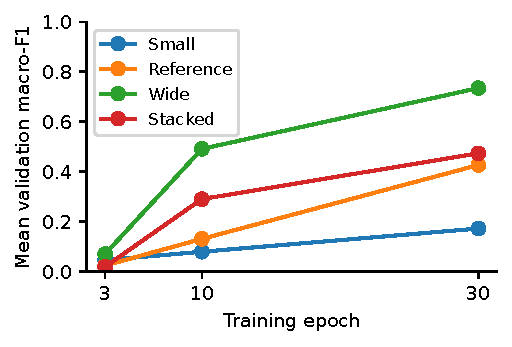
\includegraphics[width=.8\linewidth]{extended_fidelity.pdf}
\caption{Observed budget sensitivity in the fixed cohort. Four-preset behavior does not establish full-space NAS reliability.}\end{figure}
\begin{table}[htbp]\centering\small\begin{tabular}{rrrrr}
\toprule
Seed & Early epoch & Spearman & Kendall & Regret \\
\midrule
42 & 3 & 0.9487 & 0.9129 & 0.0000 \\
42 & 10 & 0.8000 & 0.6667 & 0.0000 \\
43 & 3 & 0.3162 & 0.1826 & 0.0284 \\
43 & 10 & 0.8000 & 0.6667 & 0.0000 \\
44 & 3 & 0.2000 & 0.0000 & 0.0000 \\
44 & 10 & 0.8000 & 0.6667 & 0.0000 \\
\bottomrule
\end{tabular}

\caption{Within-seed early-to-30-epoch comparisons. Regret intervals preserve ambiguity among tied early winners.}\end{table}
The cohort supplied matched candidate identities at each budget. At epoch 10, selection regret to epoch 30 was zero for all three seeds and Spearman correlation was 0.8 in every seed. At epoch 3, only seed 43 incurred positive regret, 0.0284. This cohort therefore did not establish a severe early-winner selection problem. Undefined correlations and selection-boundary ambiguities remained explicit, and no significance test was inferred from four-point correlations. The study did not complete the prespecified 25-candidate diversity study or a 200-epoch full-cohort ranking measurement. Its ranking results were measured under column L2 only.

\section{Normalization and conventional component baselines}
Column L2 used training-column norms; row L2 normalized each record; Min--Max fitted its parameters using training only. All three views retained the original random-split row IDs and the same training-fitted numeric imputation. Validation values did not fit transform parameters.

\begin{table}[htbp]\centering\begin{tabular}{lrrr}
\toprule
Scaling & Macro-F1 & Accuracy & FPR \\
\midrule
Column L2 & 0.4267 $\pm$ 0.2074 & 0.3136 & 0.9442 \\
Min--Max & 0.7831 $\pm$ 0.0768 & 0.6550 & 0.5324 \\
Row L2 & 0.7190 $\pm$ 0.0390 & 0.6710 & 0.4934 \\
\bottomrule
\end{tabular}

\caption{Reference hybrid, 30 epochs. Macro-F1 gives mean $\pm$ sample SD; accuracy and normal FPR give three-seed means.}\end{table}
\begin{figure}[htbp]\centering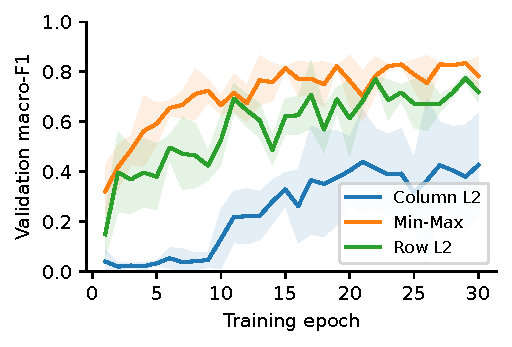
\includegraphics[width=.8\linewidth]{extended_normalization.pdf}
\caption{Reference learning curves with sample SD across training seeds. Shading is not an independent-dataset confidence interval.}\end{figure}
The mean reference macro-F1 was \ExtColumnThirty{} for column L2, \ExtRowThirty{} for row L2 and \ExtMinmaxThirty{} for Min--Max. This is evidence that a conventional scaling decision materially affected the bounded experiment. It is not evidence that normalization is a novel search contribution or that one transform dominates across releases.

The MLP used fully connected widths 64 and 32 with ReLU and dropout 0.1 after its first layer. The CNN-only control used Conv1d16, kernel 3, same padding, ReLU and pooling by 2, then flattened its features into a 32-unit ReLU head and dropout 0.1. The GRU-only control processed the feature sequence with input size 1, hidden width 32, and a dropout/classification head. These conventional baselines had different capacities and readouts. They therefore supply practical controls, not pure one-factor removal ablations.

\begin{table}[htbp]\centering\small\begin{tabular}{lrrrr}
\toprule
Model & Macro-F1 & Accuracy & FPR & Params. \\
\midrule
MLP & 0.8325 $\pm$ 0.0012 & 0.7247 & 0.4217 & 4,072 \\
CNN & 0.8275 $\pm$ 0.0032 & 0.7233 & 0.4221 & 7,016 \\
GRU & 0.7510 $\pm$ 0.0709 & 0.6416 & 0.5469 & 3,624 \\
CNN--GRU & 0.7831 $\pm$ 0.0768 & 0.6550 & 0.5324 & 5,128 \\
\bottomrule
\end{tabular}

\caption{Min--Max neural controls at 30 epochs. Parameter counts are actual model counts.}\end{table}
The MLP and CNN-only controls had higher mean validation macro-F1 than the reference hybrid at this budget. The reference's normal-class FPR was 53.24\%, while the MLP's was 42.17\%. Better macro-F1 therefore did not demonstrate acceptable operational false-alarm behavior. These controls do not establish a hybrid or NAS advantage.
\begin{table}[htbp]\centering\begin{tabular}{lrr}
\toprule
Model & Parameters & Train + validation (s) \\
\midrule
MLP & 4,072 & 13.17 \\
CNN & 7,016 & 14.23 \\
GRU & 3,624 & 16.73 \\
CNN--GRU & 5,128 & 20.14 \\
\bottomrule
\end{tabular}

\caption{Mean observed training-plus-validation elapsed seconds through epoch 30 on the GPU. Different costs mean matched epochs do not imply matched compute.}\end{table}
\begin{figure}[htbp]\centering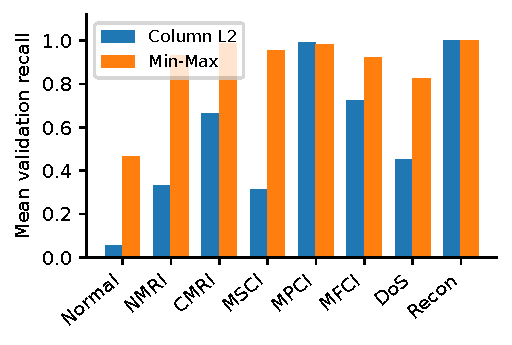
\includegraphics[width=.8\linewidth]{extended_class_recall.pdf}
\caption{Reference class recall at epoch 30, averaged across three seeds. These are validation observations, not replacements for the historical test recalls.}\end{figure}

\section{Prespecified long continuations}
Column-L2 reference trajectories for all three seeds and the Min--Max reference at seed 42 continued from epoch 30 to 200. This plan was fixed before reading new measurements. The continuations preserved model/optimizer/RNG state; they were not independent final-seed restarts.

\begin{table}[htbp]\centering\small\begin{tabular}{lrrrr}
\toprule
Scaling & Seeds & Epochs & Macro-F1 & Accuracy \\
\midrule
Column L2 & 3 & 200 & 0.8390 $\pm$ 0.0084 & 0.7267 \\
Min--Max & 1 & 200 & 0.8407 (n=1) & 0.7264 \\
\bottomrule
\end{tabular}

\caption{Actual 200-epoch validation endpoints. Min--Max has one continuation and therefore no seed-level SD.}\end{table}
\begin{figure}[htbp]\centering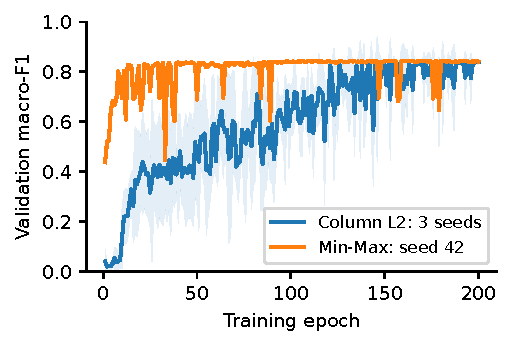
\includegraphics[width=.8\linewidth]{extended_long.pdf}
\caption{Reference trajectories through 200 epochs. The single Min--Max trajectory is explicitly distinguished from the three-seed column-L2 mean.}\end{figure}
Column L2 reached mean validation macro-F1 \ExtColumnLong{} and the one Min--Max trajectory reached \ExtMinmaxLong{}. These measurements describe longer reference-training behavior. The subsequent fixed-endpoint study reports dedicated final-seed restarts separately. Full-budget BPSO search, a complete 200-epoch architecture cohort and independently locked evaluation remain outstanding.

\section{State-grouped validation sensitivity}
Predictor-only hashes of the 25 non-time features defined groups. Labels did not define the grouping. GroupShuffleSplit used seed 1729 to reserve 20\% of groups and seed 1730 to split validation groups from the remainder. This produced 62,198 training, 14,462 validation and 20,359 reserved rows in 7,675 unique groups. Train--validation, train--reserved and validation--reserved intersections were all empty at the group level. All eight classes occurred in both training and validation.

Numeric imputation and Min--Max were fitted again on this split's training rows. The reserved partition had no exported model-input array and was not evaluated. Random forests used 100 trees and balanced class weights; logistic regression used balanced weights and training-fitted standard scaling; the reference hybrid used the same neural hyperparameters for 30 epochs on CPU. Each method used training seeds 42/43/44 on the same grouped split.

\begin{table}[htbp]\centering\begin{tabular}{llrr}
\toprule
Code & Class & Train & Validation \\
\midrule
0 & Normal & 36,140 & 8,589 \\
1 & NMRI & 1,630 & 505 \\
2 & CMRI & 10,985 & 2,222 \\
3 & MSCI & 444 & 187 \\
4 & MPCI & 4,871 & 2,456 \\
5 & MFCI & 396 & 86 \\
6 & DoS & 1,118 & 316 \\
7 & Recon & 6,614 & 101 \\
\bottomrule
\end{tabular}

\caption{Actual class support in the state-grouped training and validation partitions. Group-based fractions do not enforce equal class proportions or row fractions.}\end{table}

\begin{table}[htbp]\centering\small\begin{tabular}{lrrr}
\toprule
Model & Macro-F1 & Accuracy & FPR \\
\midrule
Random forest & 0.8372 $\pm$ 0.0010 & 0.8480 & 0.1885 \\
Logistic & 0.8018 $\pm$ 0.0000 & 0.6806 & 0.4902 \\
CNN--GRU & 0.7559 $\pm$ 0.0804 & 0.6077 & 0.6158 \\
\bottomrule
\end{tabular}

\caption{State-grouped validation results, three training seeds. Row counts and class proportions differ from the original random split.}\end{table}
The hybrid mean was \ExtGroupedHybrid{}. Zero shared exact non-time states strengthens this internal sensitivity check, but near-duplicate states and shared capture conditions may remain. The grouping is not equivalent to a capture/session split, temporal holdout or independent release. No causal claim about the amount of leakage or a prospective deployment score follows from these results.

\section{Verification and reproducibility}
The expanded CPU suite passed 74 tests, including exact continuation and test-array absence for all three newly added neural families. The new model factory leaves decoded NAS candidates on the existing hybrid path. The added controls remain outside the binary search space. The asset builder checked all 94 new measurement records against their saved validation predictions and retained prediction hashes. Training seeds and continuation endpoints were not counted as independent dataset replicates.

Run the exact studies from the repository root, using fresh output directories and an available CUDA device for the first command:
\begin{lstlisting}
python -m scripts.extend_research_evidence --device cuda --output results/research_extension
python -m scripts.state_grouped_validation --output results/state_grouped_validation
python -m scripts.build_extended_assets
\end{lstlisting}
With the bundled summaries, regenerate these figures and tables without original run directories:
\begin{lstlisting}
python -m scripts.build_extended_assets --snapshot
python3 scripts/compile_submission.py
\end{lstlisting}
The frozen settings are in \file{configs/research_extension.yaml}; individual measurements, protocols, curves and environments are included in \file{evidence/extended_*} and \file{evidence/grouped_*}. Full checkpoints remain in the local result directories. The remaining scientific actions should be read against this completed extension rather than the earlier short-budget-only status.
